\chapter{Do Judgments Screen Evidence?}

\inprog{References not even started, let alone complete, though there are hyperlinks to some of the papers I discuss. Draft only. Thanks to John Collins, Shamik Dasgupta, Adam Elga, Tom Kelly, Ishani Maitra, Ted Sider and audiences at Arch\'e for comments on earlier drafts of this paper and of its constituent parts.}

\section{Screening}

\noindent Suppose a rational agent \(S\) has some evidence \(E\) that bears on \(p\), and on that basis makes a judgment about \(p\). For simplicity, we'll normally assume that she judges that \(p\), though we're also interested in cases where the agent makes other judgments, such as that \(p\) is probable, or that \(p\) is well-supported by the evidence. We'll also assume, again for simplicity, that the agent knows that \(E\) is the basis for her judgment. Finally, we'll assume that the judgment is a rational one to make, though we won't assume the agent knows this. Indeed, whether the agent can always know that she's making a rational judgment when in fact she is will be of central importance in some of the debates that follow.

Call the proposition that the agent has made this judgment \(J\). The agent is, we'll assume, aware that \(J\) is true. She's also aware that she's rational. The fact that a rational person judges \(p\) seems to support \(p\). So it might look like \(J\) is a new piece of evidence for her, one that tells in favour of \(p\). Here then is an informal version of the question I'll discuss in this paper: \textit{How many pieces of evidence does the agent have that bear on p}? Three options present themselves.

\begin{enumerate}
\item Two - Both \(J\) and \(E\).
\item One - \(E\) subsumes whatever evidential force \(J\) has.
\item One - \(J\) subsumes whatever evidential force \(E\) has.
\end{enumerate}

\noindent This paper is about option 3. I'll call this option JSE, short for \textit{\textbf{J}udgments \textbf{S}creen \textbf{E}vidence}. I'm first going to say what I mean by screening here, and then say why JSE is interesting. Ultimately I want to defend three claims about JSE.

\begin{enumerate}
\item JSE is sufficient, given some plausible background assumptions, to derive a number of claims that have become prominent in recent epistemology (meaning approximately 2004 to the present day).
\item JSE is necessary to motivate at least some of these claims.
\item JSE is false.
\end{enumerate}

\noindent This section will largely be about saying what JSE is, and then defending 1 and 2. I'll say a bit more about 1 and 2 in the following section, focussing in detail on the role JSE plays in the Equal Weight View of disagreement. Then in sections 3 and 4, I'll develop two distinct objections to JSE.

\subsection{Screening}

The idea of screening I'm using here comes from Reichenbach's \textit{The Direction of Time}, and in particular from his work on deriving a principle that lets us infer events have a common cause. The notion was originally introduced in probabilistic terms. We say that \(C\) screens off the positive correlation between \(B\) and \(A\) if the following two conditions are met.

\begin{enumerate}
\item \(A\) and \(B\) are positively correlated probabilistically, i.e. \(Pr(A | B) > Pr(A)\).
\item  Given \(C\), \(A\) and \(B\) are probabilistically independent, \\ i.e. \(Pr(A | B \wedge C) = Pr(A | C)\).
\end{enumerate}

\noindent I'm interested in an evidential version of screening. If we have a probabilistic analysis of evidential support, the version of screening I'm going to offer here is identical to the Reichenbachian version just provided. But I want to stay neutral on whether we should think of evidence probabilistically. In general I'm somewhat sceptical of probabilistic treatments of evidence for reasons Jim Pryor goes through in his \href{http://www.jimpryor.net/research/papers/Uncertainty.pdf}{Uncertainty and Undermining}. I mention some of these in my \href{http://brian.weatherson.org/tbatd.pdf}{The Bayesian and the Dogmatist}. But I won't lean on those points in this paper.

When I say that \(C\) screens off the evidential support that \(B\) provides to \(A\), I mean the following. (Both these clauses, as well as the statement that \(C\) screens off \(B\) from \(A\), are made relative to an evidential background. I'll leave that as tacit in what follows.)

\begin{enumerate}
\item \(B\) is evidence that \(A\).
\item  \(B \wedge C\) is no better evidence that \(A\) than \(C\) is, and \(\neg B \wedge C\) is no worse evidence for \(A\) than \(C\) is.
\end{enumerate}

\noindent Here is one stylised example, and one real-world example.

Detective Det is trying to figure out whether suspect Sus committed a certain crime. Let \(A\) be that Sus is guilty, \(B\) be that Sus's fingerprints were found at the crime scene, and \(C\) be that Sus was at the crime scene when the crime was committed. Then both clauses are satisfied. \(B\) is evidence for \(A\); that's why we dust for fingerprints. But given the further evidence \(C\), then \(B\) is neither here nor there with respect to \(A\). We're only interested in finding fingerprints because they are evidence that Sus was there. If we know Sus was there, then the fingerprint evidence isn't useful one way or the other. So both clauses of the definition of screening are satisfied.

The real world example is fairly interesting. Imagine that we know Vot is an American voter in last year's US Presidential election, and we know Vot is either from \href{http://www.surveyusa.com/client/PollReport.aspx?g=29477487-154c-440d-bd34-123e584eedfb}{Alabama} or \href{http://www.surveyusa.com/client/PollReport.aspx?g=3d3e8e07-a4a1-4168-8f1e-4b8ecb26215a}{Massachusetts}, but don't know which. Let \(A\) be that Vot voted for Barack Obama, let \(B\) be that Vot is from Massachusetts, and let \(C\) be that Vot is pro-choice. Then, somewhat surprisingly, both conditions are met. Since voters in Massachusetts were much more likely to vote for Obama than voters in Alabama, \(B\) is good evidence for \(A\). But, at least according to the polls linked to the state names above, pro-choice voters in the two states voted for Obama at roughly the same rate. (In both cases, a little under two to one.) So \(C\) screens off \(B\) as evidence for \(A\), and both clauses are satisfied.

\subsection{The Idea Behind JSE}

When we think about the relation between \(J\) and \(E\), there are three conflicting pressures we immediately face. First it seems \(J\) could be evidence for \(p\). To see this, note that if someone else comes to know that \(S\) has judged that \(p\), and they know that \(S\) is as rational as them, and as well informed as them, then that could be a good reason for them to believe that \(p\). Or, at the very least, it could be evidence for them to take \(p\) to be a little more likely than they previously thought. Second, it seems like `double counting' for \(S\) to take both \(E\) and \(J\) to be evidence. After all, she only formed judgment \(J\) because of \(E\). Yet third, it seems wrong for \(S\) to simply ignore \(E\), since by stipulation, she has \(E\), and it is in general wrong to ignore evidence that one has.

The simplest argument for JSE is that it lets us accommodate all three of these ideas. \(S\) can treat \(J\) just like everyone else does, i.e. as some evidence for \(p\) without either double counting or ignoring \(E\). She can do that because she can take \(E\) to be \textit{screened off} by \(J\). That's a rather nice feature of JSE.

To be sure, it is a feature that JSE shares with a view we might call ESJ, or evidence screens judgments. That view says that \(S\) shouldn't take \(J\) to be extra evidence for \(p\), for while it is indeed some evidence for \(p\), its evidential force is screened off by \(E\). This view also allows for \(S\) to acknowledge that \(J\) has the same evidential force for her as it has for others, while also avoiding double counting. So we need some reason to prefer JSE to ESJ.

One reason (and I don't think this is what anyone would suggest is the strongest reason) is from an analogy with the fingerprint example. In that case we look for one kind of evidence, fingerprints, because it is evidence for something that is very good evidence of guilt, namely presence at the crime scene. But the thing that we are collecting fingerprint evidence for screens off the fingerprint evidence. Similarly, we might hold that we collect evidence like \(E\) because it leads to judgments like \(J\). So the later claim, \(J\) should screen \(E\), if this analogy holds up.

\subsection{JSE and Disagreement}

My main concern in this section isn't with any particular argument for JSE, but with the role that JSE might play in defending contemporary epistemological theories. I'm going to argue later that JSE is false, but first I'll argue that it is significant. I'll discuss several different ways in which JSE is implicated in contemporary work. The various theses JSE supports might not have seemed to have a lot in common, though it is notable that they have a number of proponents in common. So one of the things I'll argue is that JSE unifies some potentially disparate strands in contemporary epistemology. The primary case in which I'll be interested in concerns disagreement. Here is Adam Elga's version of the \textbf{Equal Weight View} of peer disagreement, from his \href{http://philsci-archive.pitt.edu/archive/00002940/}{Reflection and Disagreement}.

\begin{quote}Upon finding out that an advisor disagrees, your probability that you are right should equal your prior conditional probability that you would be right. Prior to what? Prior to your thinking through the disputed issue, and finding out what the advisor thinks of it. Conditional on what? On whatever you have learned about the circumstances of the disagreement.\end{quote}

\noindent It is easy to see how JSE could lead to some kind of equal weight view. If your evidence that \(p\) is summed up in your judgment that \(p\), and another person who you regard as equally likely to be right has judged that \(\neg p\), then you have exactly the same kind of evidence for \(p\) as against it.  So you should suspend judgment about whether \(p\) is true or not. In section 2 I'll discuss how to turn this informal idea into a full argument.

But for now I want to focus on the  role that JSE can play is in the clause about priority. Here is one kind of situation that Elga wants to rule out. \(S\) has some evidence \(E\) that she takes to be good evidence for \(p\). She thinks \(T\) is an epistemic peer. She then learns that \(T\), whose evidence is also \(E\), has concluded \(\neg p\). She decides, simply on that basis, that \(T\) must not be an epistemic peer, because \(T\) has got this case wrong. This decision violates the Equal Weight View, because it uses \(S\)'s probability that \(T\) is a peer \textit{after} thinking through the disputed issue, not prior to this, in forming her judgment about how likely it is that she was right, i.e., how likely it is that \(p\) is true.

Now at first it might seem that \(S\) isn't doing anything wrong here. If she knows how to apply \(E\) properly, and can see that \(T\) is misapplying it, then she has good reason to think that \(T\) isn't really an epistemic peer after all. She may have thought previously that \(T\) was a peer, indeed she may have had good reason to think that. But she now has excellent evidence, gained from thinking through this very case, to think that \(T\) is not a peer, and so not worthy of deference.

Since Elga thinks that there is something wrong with this line of reasoning, there must be some way to block it. I think by far the best option for blocking it comes from ruling that \(E\) is not available evidence for \(S\) once she is using \(J\) as a judgment. That is, the best block available seems to me to come from JSE. For once we have JSE in place, we can say very simply what is wrong with \(S\) here. She is like the detective who says that we have lots of evidence that Sus is guilty--not only was she at the crime scene, but her fingerprints were there. To make the case more analogous, we might imagine that there are detectives with competing theories about who is guilty in this case. If we don't know who was at the crime scene, then fingerprint evidence may favour one detective's theory over the other. If we do know that both suspects were known to be at the crime scene, then fingerprint evidence isn't much help to either.

So I think that if JSE is true, we have an argument for Elga's strong version of the Equal Weight View, one which holds agents are not allowed to use the dispute at issue as evidence for or against the peerhood of another. And if JSE is not true, then there is a kind of reasoning which undermines Elga's Equal Weight View, and which seems, to me at least, unimpeachable. So I think Elga's version of the Equal Weight View requires JSE, and JSE is at least arguably sufficient for Elga's version of the Equal Weight View.

That last claim might look too strong in a couple of respects. On the one hand, we might worry that we could accept JSE and still reject the Equal Weight View because of epistemic partiality. Here's a way to do that. Say we thought that \(S\) should given more weight to \(T_1\)'s judgment than \(T_2\)'s judgment if \(S\) stands in a special relationship to \(T_1\) and not to \(T_2\), even if \(S\) has no reason independent of the relationship to believe that \(T_1\) is more reliable. And say that \(S\) stands in that relationship to herself. Then \(S\)'s own judgment that \(p\) might be better evidence for her that \(p\) than a peer's judgment. The view I've just sketched is a schema; it becomes more precise when we fill in what the relationship is. Ralph Wedgwood has proposed a version of this view where the special relationship is \textit{identity}. Sarah Stroud has proposed a version of this view where the special relationship is \textit{friendship}. For what it's worth, I'm a little sceptical of such views, but arguing against them would take us too far away from our main goal. Instead I'll just note that if you do like such views, you should agree with me that JSE is necessary to motivate the Equal Weight View, and disagree that it's sufficient. Put another way, the falsity of such views is a needed extra premise to get that JSE is necessary and sufficient for the Equal Weight View.

For somewhat different reasons, considering the details of JSE might make us worry that JSE is not strong enough to support a full-blooded version of the Equal Weight View. After all, JSE was restricted to the case where the agent's judgment is rational. So all it could support is a version of the Equal Weight View restricted to agents who initially make a rational judgment. But I think this isn't actually a problem, since we need to put some kind of restriction on Equal Weight in any case. We need to put such a restriction on because the alternative is to allow a kind of epistemic laundering.

Consider an agent who makes an irrational judgment. And assume her friend, who she knows to be a peer, makes the same irrational judgment. What does the Equal Weight View say she should do? It should be bad for it to say that she should regard her and her friend as equally likely to be right, so she should keep this judgment. After all, it was irrational! There are a couple of moves the friend of the Equal Weight View can make at this point. But I think the simplest one will be to put some kind of restriction on Equal Weight. If that restriction is to agents who have initially made rational judgments, then it isn't a problem that JSE is restricted in the same way. 

\subsection{White on Permissiveness}

In his 2005 \textit{Philosophical Perspectives} paper, \href{http://philosophy.fas.nyu.edu/docs/IO/1180/EP.pdf }{Epistemic Permissiveness}, Roger White argues that there cannot be a case where it could be epistemically rational, on evidence \(E\), to believe \(p\), and also rational, on the same evidence, to believe \(\neg p\). One of the central arguments in that paper is an analogy between two cases.

\begin{quote}
\textbf{Random Belief}: \(S\) is given a pill which will lead to her forming a belief about \(p\). There is a \(\nicefrac{1}{2}\) chance it will lead to the true belief, and a \(\nicefrac{1}{2}\) chance it will lead to the false belief. \(S\) takes the pill, forms the belief, a belief that \(p\) as it turns out, and then, on reflecting on how she formed the belief, maintains that belief.

\textbf{Competing Rationalities}: \(S\) is told, before she looks at \(E\), that some rational people form the belief that \(p\) on the basis of \(E\), and others form the belief that \(\neg p\) on the basis of \(E\). \(S\) then looks at \(E\) and, on that basis, forms the belief that \(p\).
\end{quote}

\noindent White claims that \(S\) is no better off in the second case than in the former. As he says,

\begin{quote}
Supposing this is so, is there any advantage, from the point of view of pursuing the truth, in carefully weighing the evidence to draw a conclusion, rather than just taking a belief-inducing pill? Surely I have no better chance of forming a true belief either way.
\end{quote}

\noindent But it seems to me that there is all the advantage in the world. In the second case, \(S\) has evidence that tells on \(p\), and in the former she does not. Indeed, I long found it hard to see how we could even think the cases are any kind of analogy. But I now think JSE holds the key to the argument.

Assume that JSE is true. Then after \(S\) evaluates \(E\), she forms a judgment, and \(J\) is the proposition that she formed that judgment. Now it might be true that \(E\) itself is good evidence for \(p\). (The target of White's critique says that \(E\) is also good evidence for \(\neg p\), but that's not yet relevant.) But given JSE, that fact isn't relevant to \(S\)'s current state. For her evidence is, in its entirity, \(J\). And she knows that, as a rational agent, she could just as easily have formed some other judgment, in which case \(J\) would have been false. Indeed, she could have formed the opposite judgment. So \(J\) is no evidence at all, and she is just like the person who forms a random belief, contradicting the assumption that believing \(p\) could, in this case, be rational, and that believing \(\neg p\) could be rational.

Without JSE, I don't see how White's analogy holds up. There seems to be a world of difference between forming a belief via a pill, and forming a belief on the basis of the evidence, even if you know that other rational agents take the evidence to support a different conclusion. In the former case, you have violated every epistemic rule we know of. In the latter, you have reasons for your belief, you can defend it against challenges, you know how it fits with other views, you know when and why you would give it up, and so on. The analogy seems worse than useless by any of those measures.

\subsection{Christensen on Higher-Order Evidence}

Next, I'll look at some of the arguments David Christensen brings up in his \href{http://www.brown.edu/Departments/Philosophy/faculty/christensen/Higher-OrderEvidence.pdf}{Higher Order Evidence}. Christensen imagines a case in which we are asked to do a simple logic puzzle, and are then told that we have been given a drug which decreases logical acumen in the majority of people who take it. He thinks that we have evidence against the conclusions we have drawn.

Let's consider a particular version of that, modelled on Christensen's example of Ferdinand the bull. \(S\) knows that \(\forall x (Fx \rightarrow Gx)\) , and knows that \(\neg (Fa \wedge Ga)\). \(S\) then infers deductively that \(\neg Fa\). \(S\) is then told that she's been given a drug that dramatically impairs abilities to draw deductive conclusions. Christensen's view is that this testimony is evidence against  \(\neg Fa\), which I assume implies that it is evidence that \(Fa\).

This looks quite surprising. \(S\) has evidence which \textbf{entails} that \(\neg Fa\), and her evidence about the drug doesn't rebut that evidence. It does, says Christensen, undermine her evidence for \(\neg Fa\). But not because it undermines the entailment; it isn't like the evidence gives her reason to believe some non-classical logic where this entailment does not go through is correct. So how could it be an underminer?

Again, JSE seems to provide an answer. If \(S\)'s evidence that \(\neg Fa\) is ultimately just her judgment that it is entailed by her other evidence, and that judgment is revealed to be unreliable because of her recent medication, then \(S\) does lose evidence that \(\neg Fa\). But if we thought the original evidence, i.e., \(\forall x (Fx \rightarrow Gx)\) and \(\neg (Fa \wedge Ga)\), was still available to \(S\), then there is a good reason to say that her evidence conclusively establishes that \(\neg Fa\).

Note that I'm not saying here that Christensen argues from JSE to his conclusion. Rather, I'm arguing that JSE delivers the conclusion Christensen wants, and without JSE there seems to be a fatal flaw in his argument. So Christensen's view needs JSE as well.

\subsection{Egan and Elga on Self-Confidence}

Finally, I'll look at some conclusions that Andy Egan and Adam Elga draw about self-confidence in their paper \href{http://philsci-archive.pitt.edu/archive/00002432/}{I Can't Believe I'm Stupid}. I think many of the conclusions they draw in that paper rely on JSE, but I'll focus just on the most prominent use of JSE in the paper.

\begin{quote}
One of the authors of this paper has horrible navigational instincts. When this author---call him ``AE''---has to make a close judgment call as to which of two roads to take, he tends to take the wrong road.  If it were just AE's first instincts that were mistaken, this would be no handicap.  Approaching an intersection, AE would simply check which way he is initially inclined to go, and then go the opposite way.  Unfortunately, it is not merely AE's first instincts that go wrong: it is his all things considered judgments.  As a result, his worse-than-chance navigational performance persists, despite his full awareness of it.  For example, he tends to take the wrong road, even when he second-guesses himself by choosing against his initial inclinations.

Now: AE faces an unfamiliar intersection.  What should he believe about which turn is correct, given the anti-reliability of his all-things-considered judgments?  Answer: AE should suspend judgment.  For that is the only stable state of belief available to him, since any other state undermines itself.  For example, if AE were at all confident that he should turn left, that confidence would itself be evidence that he should \textit{not} turn left.  In other words, AE should realize that, were he to form strong navigational opinions, those opinions would tend to be mistaken.  Realizing this, he should refrain from forming strong navigational opinions (and should outsource his navigational decision-making to someone else whenever possible)
\end{quote}

\noindent I think that this reasoning goes through iff JSE is assumed. I'll argue for this by first showing how the reasoning could fail without JSE, and then showing how JSE could fix the argument.

Start with a slightly different case. I am trying to find out whether \(p\), where this is something I know little about. I ask ten people whether \(p\) is true, each of them being someone I have good reason to believe is an expert. The experts have a chance to consult before talking to me, so each of them knows what the others will advise. Nine of them confidently assure me that \(p\) is true. The tenth is somewhat equivocal, but says that he suspects it is not, although he cannot offer any reasons for this that the other nine have not considered. It seems plausible in such a case that I should, or at least may, simply accept the supermajority's verdict, and believe \(p\).

Now change the case a little. The first nine are experts, but the tenth is something of an anti-expert. He is wrong considerably more often than not on these matters. Again, the first nine confidently assert that \(p\). In this case, the tenth is equally confident that \(p\). My epistemic situation looks much like it did in the previous paragraph. I have a lot of evidence for \(p\), and a little evidence against it. The evidence against has changed a little; it is now the confident verdict of a sometimes anti-expert, rather than the equivocal anti-verdict of an expert, but this doesn't look like a big difference all-things-considered. So I still should, or at least may, believe \(p\).

Now make one final change. I am the tenth person consulted. I ask the first nine people, who of course all know each other's work, and they all say \(p\). I know that I have a tendency to make a wrong judgment in this type of situation -- even when I've had a chance to consult with experts. (Perhaps \(p\) is the proposition that the right road is to the left, and I am AE, for example. It does require some amount of hubris to continue to be an anti-expert even once you know you are one, and the judgments are made in the presence of expert advise. But I don't think positing delusionally narcissistic agents makes the case unrealistic.) After listening to the experts, I judge that \(p\). This is some evidence that \(\neg p\), since I'm an anti-expert. But, as in the last two paragraphs, it doesn't seem that it should override all the other evidence I have. So, even if I know that I'm in general fairly anti-reliable on questions like \(p\), I need not suspend judgment. On those (presumably rare) occasions where my judgment tracks the evidence, I should keep it, even once I acknowledge I have made the judgment.

The previous paragraph assumed that JSE did not hold. It assumed that I could still rely on the nine experts, even once I'd incorporated their testimony into a judgment. That's what JSE denies. According to JSE, the arguments of the previous paragraph rely on illicitly basing belief on screened-off evidence. That's bad. If JSE holds, then once I make a judgment, it's all the evidence I have. Now assume JSE is true, and that I know myself to be something of an anti-expert. Then any judgment I make is fatally self-undermining, just like Egan and Elga say. When I make a judgment, I not only have evidence it is false, I have undefeated evidence it is false. So if I know I'm an anti-expert, I must suspect judgment. That's the conclusion Egan and Elga draw, and it seems to be the right conclusion iff JSE is true. So the argument here relies on JSE. 

\section{Why JSE matters}

I've argued that Adam Elga's version of the Equal Weight View of disagreement, Roger White's view of permissiveness, David Christensen's view of higher-order evidence, and Andy Egan and Adam Elga's view of self-confidence, all stand or fall with JSE. Not surprisingly, Christensen also has a version of the Equal Weight View of evidence, and, as Tom Kelly notes in his \href{http://www.princeton.edu/~tkelly/papers/KellyPeerDis-1.doc}{Peer Disagreement and Higher-Order Evidence}, there is a strong correlation between holding the Equal Weight View, and rejecting epistemic permissiveness. So I don't think it is a coincidence that these views stand or fall with JSE. Rather, I think JSE is a common thread to the important work done by these epistemologists on disagreement, permissiveness and higher-order evidence.

This isn't surprising; in fact it is hard to motivate these theories, especially the Equal Weight View, without JSE. (The arguments about permissiveness are a little distinct from the arguments about disagreement and higher-order evidence, since there I'm only responding to one kind of argument against permissiveness, and there may be other arguments against permissiveness that have a very different structure, and hence are not connected to JSE.) I already noted that there's a very strong response to the Equal Weight View available if the JSE is false. But even if you didn't like that response, without the JSE the Equal Weight View doesn't really seem to have much motivation at all. Let's consider what happens in a situation of peer disagreement without JSE, remembering that we argued earlier that JSE was sufficient to ground the Equal Weight Hypothesis.

In a typical situation of peer disagreement, agent \(A\) has evidence \(E\), and on that basis comes to a judgment that \(p\). (Perhaps she isn't so decisive, but we'll work with this kind of case for simplicity.) As always, let \(J\) be that that judgment was made. And let's assume that it was a rational judgment to make on the basis of \(E\), and that \(A\) knows both that she's made the judgment and that she's a generally rational person. Then \(B\), a peer of \(A\), makes a conflicting judgment, say that \(\neg p\), and \(A\) comes to know about this. What should \(A\) do?

If JSE is false, then \(A\) has two pieces of evidence in favour of \(p\). She has \(E\), and she has the fact that she, a generally rational person, judged \(p\). And she has one piece of evidence against \(p\), namely the fact that \(B\) made a conflicting judgment \(\neg p\). Two of these pieces of evidence look like they might cancel each other out, namely the two judgments. But there's one more piece of evidence available for \(p\), namely \(E\). If JSE is false, that means \(A\) has a reason to be more confident in \(p\) that in \(\neg p\). And that means that the Equal Weight View is false, since the Equal Weight View says that \(A\) has no reason to be more confident in \(p\) that in \(\neg p\).

The argument here is intended to complement the earlier discussion of disagreement with and without JSE. Earlier I argued that without JSE agents can use the fact of disagreement to conclude that someone who seemed to be a peer is not in fact a peer. If that's right, then they might use \(E\) to simply not change their mind at all. Here I'm arguing that even if they accept that the other person is a peer, without JSE that's compatible with not being `balanced' between \(p\) and \(\neg p\). Surprisingly, this is so even if they give their own judgment and their peer's judgment `equal weight'; the tie-breaker is \(E\) itself, which is not a judgment.

To be sure, on this line of reasoning, it isn't obvious that \(A\) should stay firmly wedded to \(p\). There's a difference between having one uncontested reason to judge \(p\), versus having two reasons to judge \(p\) and one to judge \(\neg p\). In the latter case, perhaps it is reasonable to have a more tentative attitude towards \(p\). But what seems to come through clearly is that with JSE we have a strong argument for the Equal Weight View, and without JSE the Equal Weight View is not motivated, while an objection to it is motivated. So the JSE is tied very closely to the Equal Weight View.

\subsection{Varieties of Defeaters}

\noindent It might be worried that the argument of the previous section ignores the distinction between rebutting and undercutting defeaters. The proponent of the Equal Weight View might hold that in the situation I've described, \(B\)'s judgment \(\neg p\) is both a rebutting defeater with respect to \(A\)'s judgment \(p\), since it directly provides reason for an alternative judgment, and an undercutting defeater with respect to the support \(E\) provides for \(p\), since it provides reason to think that \(E\) does not really support \(p\). If that is the right way to think about things, then it is misleading to simply count up the two reasons in favour of \(p\) versus one reason against, since \(A\)'s judgment and \(B\)'s judgment have different effects.

I think the right thing to do at this point is to get a little clearer on just what exactly undercutting defeaters are supposed to do. In general, an undercutting defeater purports to tell us that some evidence \(E\) is not good evidence for a conclusion \(H\). This suggests a picture of how undercutting defeaters work. If \(D\) undercuts the inference from \(E\) to \(H\), but does not rebut that inference, that's because (a) \(D\) is a rebutting defeater for the agent's previous belief that \(E\) supports \(H\), and (b) the inference from \(E\) to \(H\) is reasonable if it is sufficiently rebutted.

It's important to draw a distinction between first-order and second-order justification here. The picture I'm suggesting is that undercutting defeaters are in the first instance rebutting defeaters for the claim that the agent is justified in believing \(H\). That is, when the agent gets an undercutting defeater, the first thing that happens is that the \textit{second-order} claim that the agent is justified in believing she is justified in believing \(H\) becomes false. What effect does this have on the first-order claim that the agent is justified in believing \(H\)? That, I'm going to argue, depends on the nature of the relationship between \(E\) and \(H\).

In normal caes, if you aren't justified in believing that \(E\) supports \(H\), then you aren't justified in inferring \(H\) from \(E\). If I don't know that a particular kitchen scale is reliable, and so don't know whether an agent is justified in believing what it says, then plausibly I'm not justified in inferring from the fact that it says that \(p\) to \(p\). But that's not because there's a general rule that first-order justification, in this case believing \(p\), requires second-order justification, in this case being justified in believing I'm justified in believing \(p\). Rather, it's because for non-basic inferential methods, we are only justified in using them if we are justified in believing they are sound. Regress arguments, of the kind Lewis Carroll alludes to in ``Achilles and the Tortoise'', suggest that can't be right for \textit{basic} inferential methods. 

The regress arguments suggest that at some level we must have unjustified justifiers. One natural place to find such things, indeed the place Carroll suggests they are located, is in basic inferential rules. For instance, if classical logic is the correct logic, then plausibly the rule that says an agent is justified in inferring \(H\) from \(\neg \neg H\) is basic. And by this, I mean that an agent can infer \(H\) from \(\neg \neg H\) even if she has no antecedent reason to believe that this inference is justified.

Now we have to be a little careful here.\footnote{I'm grateful to several people, including Shamik Dasgupta, Thomas Kelly and Ted Sider, for pointing out how I was not being quite so careful in an earlier draft of this paper.} What the regress arguments show is that we need unjustified justifiers. They don't show that we need \textit{indefeasible} justifiers. So even if our agent the inference from  \(\neg \neg H\)  to \(H\) is basic, that doesn't mean it can't be defeated by some evidence. There's a useful comparison to be made here to James Pryor's dogmatist theory of perception. Pryor says that we can trust our senses in the absence of reason to believe that they are reliable. But he doesn't say, and it would be a somewhat implausible thing to say, that we can trust our senses in the presence of reason to believe they are unreliable. A kind of dogmatism about basic inference, one that says basic inferences do not need to be justified but can be defeated, seems like a plausible and natural parallel.

This theory about basic inferences has some consequences for the theory of undercutting defeaters. Assume that the inference from \(E\) to \(H\) is basic. And assume that an agent who has \(E\), and who had previously inferred \(H\), gets a relatively weak undercutting defeater for this inference. I claim that in some such cases, she might still be justified in believing \(H\), because the original inference was basic. What I mean by a relatively weak undercutting defeater is that when the agent gets the defeater, she is no longer justified in believing that she is justified in inferring \(H\) from \(E\), but nor is she justified in believing she is unjustified in inferring \(H\) from \(E\). Now if the inference from \(E\) to \(H\) can only be properly made by someone who knows it is a good inference, then the agent can't properly make that inference. So in that case the undercutting defeater does defeat the agent's justification. But I've argued that this extra premise, about the inference requiring that the agent know it is a good one, is not true when the inference is basic. So if the inference from \(E\) to \(H\) is basic, and the agent gets this undercutting defeater, then she is still justified in making the inference. So she is justified in believing \(H\). But she is no longer justified in believing that she has got to \(H\) by a justified route, so she is not justified in believing that she is justified in believing \(H\).

I think that at least some of the time, that's what happens in disagreement. If we infer \(p\) from some evidence, and our friend refuses to make this inference, that undercuts our belief in \(p\). That is, it rebuts our prior belief that \(p\) is supported by this evidence. In most cases, that will be enough to make our belief in \(p\) unjustified. But at least some of the time, we can infer \(p\) from some evidence even if we are not justified in believing \(p\) is supported by that evidence. In those cases, the Equal Weight View is unmotivated.

The treatment of undercutting defeaters I've just offered, as rebutting defeaters of claims about justification, assumes that what we should believe can come apart from what we should believe that we should believe. Some people might find that assumption intolerable. So the rest of this section is devoted to arguing that it is true.

\subsection{Misleading Evidence in Ethics and Epistemology}

Among the many things we don't know include many truths about ethics. The existence of many intelligent philosophers promoting false theories doesn't help much. (Since ethicists disagree with one another, I'm pretty sure many of them are saying false things!) There have been several recent works on what the \textit{moral} significance of moral uncertainty is (e.g., Sepielli, Lockhart). I'm inclined to think that it isn't very great, although moral uncertainty might have some very odd \textit{epistemological} consequences in cases like the following.

\begin{quote} \textbf{Kantians}: Frances believes that lying is morally permissible when the purpose of the lie is to prevent the recipient of the lie performing a seriously immoral act. In fact she's correct; if you know that someone will commit a seriously immoral act unless you lie, then you should lie. Unfortunately, this belief of Frances's is subsequently undermined when she goes to university and takes courses from brilliant Kantian professors. Frances knows that the reasons her professors advance for the immorality of lying are much stronger than the reasons she can advance for her earlier moral beliefs. After one particularly brilliant lecture, Frances is at home when a man comes to the door with a large axe. He says he is looking for Frances's flatmate, and plans to kill him, and asks Frances where her flatmate is. If Frances says, ``He's at the police station across the road", the axeman will head over there, and be arrested. But that would be a lie. Saying anything else, or saying nothing at all, will put her flatmate at great risk, since in fact he's hiding under a desk six feet behind Frances. What should she do? \end{quote}

\noindent That's an easy one! The text says that unless someone will commit a seriously immoral act unless you lie, you should lie. So Frances should lie. The trickier question is what she should believe. I think she should believe that she'd be doing the wrong thing if she lies. After all, she has excellent evidence for that, from the testimony of the ethical experts, and she doesn't have compelling defeaters for that testimony. So she should do something that she believes, and should believe, is wrong. That's OK; by hypothesis her Kantian professors are wrong about what's right and wrong. 

So I think the immediate questions about what Frances should do and believe are easy. But the result is that Frances is in a certain way incoherent. For her to be as she should, she must do something she believes is wrong. That is, she should do something even thought she should believe that she should not do it. So I conclude that it is possible that sometimes what we should do is the opposite of we should believe we should do.

If we've gone this far, we might be tempted by an analogy between ethics and epistemology. The conclusion of this analogy is that sometimes what we should believe is different from what we should believe that we should believe. This is what would follow if we believe the conclusion of the previous paragraph, and we think that whatever is true of action is (or at least probably is) true of belief as well.

It might be objected here that there is a big disanalogy between ethics and epistemology. The objector says that since actions are voluntary, but beliefs are voluntary, we shouldn't expect the norms for the two to be the same. I think this objection fails twice over. I've argued elsewhere that beliefs are much more like actions in terms of their normative status than is usually acknowledged (\href{http://brian.weatherson.org/DDD.pdf}{Deontology and Descartes' Demon}). But I won't rely on that here. Because I think the simpler point to notice is that if there is a disanalogy between ethics and epistemology, it works \textit{in favour} of the position I'm taking.

I'm trying to argue that it's possible to justifiably believe \(p\) on the basis of \(E\) even though you don't have reason to believe that \(E\) supports \(p\), indeed even if you have reason to believe that \(E\) does not support \(p\). That is, I'm trying to argue that which first-order beliefs it is rational to have can come apart from which beliefs it is rational to have about which first-order beliefs it is rational to have. And I've argued so far that which actions you have most reason to do can come apart from which beliefs it is rational to have about which actions you have most reason to do. 

Now if there's a reason that these `first-order' and `second-order' states should line up, it's presumably because you should, on reflection try to get your relations to the world into some kind of broad coherence. But that's a kind of consideration that applies much more strongly to things that we do after considered reflection, like lie to the murderer, than it does to things we do involuntarily, like form beliefs.\footnote{As I mentioned earlier, I don't really think this is the right picture of belief formation, but I'm taking it on board for the sake of considering this objection.} Put another way, when we are considering the norms applicable to involuntary bodily movements, we generally settle on fairly externalist considerations. A good digestive system, for instance, is simply one that digests food well, not one that digests in accord with reason, or in a coherent manner given other bodily movements, or anything of the sort. So if beliefs are involuntary, we should think they are to be judged more on how they line up with reality, and less on how well they cohere to our broader worldview. But that's to say we should care \textit{less} about coherence between beliefs and beliefs about doxastic normativity than we do about coherence between action and beliefs about norms of action. So if there's a disanalogy between ethics and epistemology here, it's one that makes my position stronger, not weaker.

There is one disanalogy between the ethical case and the epistemological case that's a little harmful to my case, though I don't think it's a particularly strong disanalogy. In both cases there are two modal operators. In the epistemological case, they are both epistemic modals: I claim the agent can be justified in believing \(p\) although she's not justified in believing she's justified in believing \(p\). In the moral case, one is deontic and one is epistemic: I claim the agent can be justified in doing \(\phi\) even though she's not justified in believing she's justified in doing \(\phi\). This doesn't seem like a particularly serious difference between the cases to me, but if you do, you'll be less impressed by this argument from analogy.

The upshot of this is that I think that the argument by analogy is a good argument for my preferred way of treating undermining defeaters. But even if you think the argument can't bear all that weight, the analogy does help with deflecting some arguments against the position I'm defending. The arguments I have in mind are those proffered by Richard Feldman in ``Respecting the Evidence''. He thinks that we can't rationally be in a position where we believe \(p\) on the basis of \(E\), and we know \(E\) is our basis for \(p\), and yet we have good (if misleading) grounds for believing \(E\) does not support \(p\). Here's his setup of the debate.

\begin{quote}
Consider a person who has some evidence, \(E\), concerning a proposition, \(p\), and also has some evidence about whether \(E\) is good evidence for \(p\). I will say that the person is \textit{respecting the evidence} about \(E\) and \(p\) when the person's belief concerning \(p\) corresponds to what is indicated by the person's evidence about \(E\)'s support for \(p\). That is, a person respects the evidence about \(E\) and \(p\) by believing \(p\) when his or her evidence indicates that this evidence supports \(p\) or by not believing \(p\) when the evidence indicates that this evidence does not support \(p\). (Feldman 2005: 95-6)
\end{quote}

\noindent Feldman goes on to argue that we should respect the evidence. Obviously I disagree. If \(E\) is all the agent's evidence, then the agent's attitude towards \(p\) should be determined by how strongly \(E\) supports \(p\). One case that strongly suggests this is when the agent has no evidence whatsoever about how \(E\) supports \(p\), so the agent's evidence indicates nothing about \(E\)'s support for \(p\). If that implies that the agent can't have any attitudes about \(p\), then we are led quickly into an unpleasant regress.

But the main point I want to make here concerns the arguments that Feldman makes for respecting the evidence. It is true that sometimes disrespecting the evidence has counterintuitive consequences. See, for example, Feldman's example of the baseball website (Feldman 2005: 112) or, for that matter, the discussion of kitchen scales in the previous subsection. But other cases might point the other way. Is it really intuitive that the student can't soundly infer \(p\) from \(\neg \neg p\) after hearing some lectures from a talented but mistaken intuitionistic logician? I think intuition is sufficiently confused here that we should rely on other evidence. Feldman's primary argument concerns the oddity of the position I'm defending. In his taxonomy of views, `View 1' is the view that when an agent has evidence \(E\), which is in fact good evidence for \(p\), and gets misleading evidence that \(E\) does not in fact support \(p\), then she can know \(p\), but not know that she knows \(p\). That's what I think happens at least some of the time, at least when the connection between \(E\) and \(p\) is basic, so his arguments are meant to tell against my position.

\begin{quote}
View 1... has the implication that a person could be in a situation in which she justifiably denies or suspends judgment about whether her basis for believing a proposition is a good one, but nevertheless justifiably believes the proposition. Imagine such a person reporting her situation: ``\(p\), but of course I have no idea whether my evidence for \(p\) is any good.'' At the very least, this sounds odd. (Feldman 2005: 105)
\end{quote}

\noindent He later goes into more detail on this point.

\begin{quote}
View 1 leads to the conclusion that our student can correctly believe things such as

\begin{enumerate}
\setcounter{enumi}{5}
\item \(T\), but my overall evidence does not support \(T\).
\end{enumerate}

\noindent ... As noted, (6) seems odd. No doubt things like (6) can be true. And it may be that (6) does not have quite the paradoxical air that ``\(T\), but I don't believe \(T\)'' has. Still, when the student acknowledges in the second conjunct that her evidence does not support \(T\), she says that she does not have good reason to assert the first conjunct. So, if she is right about the second conjunct, her evidence does not support the first conjunct. Thus, if reasonable belief requires evidential support, it is impossible for the student's belief in (6) to be both true and reasonable. And, if knowledge requires truth and reasonable belief, it also follows that she cannot know (6). While it does not follow that belief in (6) cannot be reasonable, it does make it peculiar. One wonders what circumstances could make belief in it reasonable. (Feldman 2005: 108-9)
\end{quote}

\noindent The last line is easy to reply to. The circumstances that could make it reasonable are ones where the agent has good evidence that \(T\), but also has misleading evidence about the quality of her evidence. 

The more substantial point concerns the reasonableness of believing (6). As Feldman notes, the issue is not whether the subject could \textit{truly} believe (6). In the circumstances we're interested in, the second conjunct of (6) is false, although well supported by evidence. So the issue is just whether it could be a justified belief. To make the argument that it could not be justified work, Feldman needs to thread a very tight normative needle. If we say that a belief must actually constitute knowledge to be justified, then my view does not have the consequence that an agent could justifiably believe (6). That's simply because the second conjunct is false. On the other hand, if justification does not require knowability, then it isn't clear why the belief in (6) is not justified. By hypothesis, each conjunct is well supported by the evidence. So we only get a problem if justification requires knowability, but not knowledge. And there's no reason, I think, to hold just that position; it makes the relation between justification and knowledge just too odd.

And while there is something disarming about the conjunction, reflection on cases like Kantians should remind us that there's nothing too odd about the two conjuncts. Frances should lie to the murderer at the door, and she should believe that she has most reason to not lie to the murderer at the door. That doesn't seem too different from it being the case that she should believe \(p\), and she should believe that she has most reason to not believe \(p\). And, assuming a natural connection between evidence and reason, that in turn isn't very different from it being the case that she should believe \(p\), and she should believe that her evidence does not support \(p\). Given that cases like Frances' exist, it isn't odd that someone could be in a postion to reasonably believe each conjunct of (6). So, contra Feldman, it isn't odd that they could be in a position to reasonably believe (6). 

So I conclude that undercutting defeaters give us reason to think our evidence does not support a particular hypothesis, and this sometimes, but not all the time, gives us reason to lower our confidence in that hypothesis. And as I've argued above, on that picture of how undercutting defeaters work, there is no JSE-free argument for the Equal Weight View. Indeed, if that's how undercutting works, then if JSE is not assumed, it seems the Equal Weight View really requires that the peer's judgment do double duty, both overriding our judgment and overriding the initial evidence. And that's not a very intuitive picture.

\section{JSE and Practical Action}
As we noted earlier, Christensen's position on higher-order evidence is closely related to JSE. Indeed, some of the examples he uses to motivate his claim about higher-order evidence seem also to provide motivation for JSE. In a number of cases that he offers, evidence about the circumstances in which a judgment is made provide reason, he says, for the judger to lower her confidence in a certain proposition, even if that initial judgment was correct. I'm going to argue that if Christensen is right, we should also expect to find cases where evidence about the circumstances in which the judgment is made provide reason for the judger to \textit{raise} her confidence in a certain proposition, even if once again that initial judgment was correct. And, I'll argue, that's not what investigation of the cases reveals. But first let's look two of at Christensen's examples. (I've slightly changed the numbers in the second case.)

\begin{quote} \textbf{Sleepy Hospital}: I'm a medical resident who diagnoses patients and prescribes appropriate treatment.  After diagnosing a particular patient's condition and prescribing certain medications, I'm informed by a nurse that I've been awake for 36 hours.  I reduce my confidence in my diagnosis and prescription, pending a careful recheck of my thinking. \end{quote}

\begin{quote} \textbf{Tipping}: My friend and I have been going out to dinner for many years.  We always tip 20\% and divide the bill equally, and we always do the math in our heads.  We're quite accurate, but on those occasions on which we've disagreed in the past, we've been right equally often. This evening seems typical, in that I don't feel unusually tired or alert, and neither my friend nor I have had more wine or coffee than usual.  I get \$42 in my mental calculation, and become quite confident of this answer.  But then my friend says she got \$45. I dramatically reduce my confidence that \$42 is the right answer, and dramatically increase my confidence that \$45 is correct, to the point that I have roughly equal confidence in each of the two answers.  \end{quote}

\noindent Christensen thinks the things the narrator does in each case are, all things considered, the right thing to do. We should note to start with that there's something a little odd about this. This is easiest to see in \textbf{Tipping}. Let's say the bill was \$70. Then the narrator's share was \$70 $\div$ 2, i.e. \$35 plus 20\% for the tip, so plus \$7, so it is \$42. The narrator is competent with simple arithmetic, so he has access to all of this evidence, and not believing something that is clearly entailed by one's evidence is bad, especially when you are trying to figure out whether it is true and have worked through the computation. But Christensen thinks it is even worse to, immodestly, take oneself to be the one who is correct in a dispute like this. His primary motivation for this, I think, comes from the following variant on Sleepy Hospital.

\begin{quote}Or consider the variant where my conclusion concerns the drug dosage for a critical patient, and ask yourself if it would be morally acceptable for me to write the prescription without getting someone else to corroborate my judgment.  Insofar as I'm morally obliged to corroborate, it's because the information about my being drugged should lower my confidence in my conclusion. (Christensen, pg 11) \end{quote}

I think the last line here isn't correct. Indeed, I think the last line reveals a crucial premise connecting belief and action that is at the heart of his argument, and which is mistaken. In the example, the medical evidence suggests that the prescription should be, let's say, 100$\mu$g, and that's what the narrator at first intends to prescribe. But the narrator also has evidence that he's unreliable at the moment, since he's been awake so long. Christensen thinks that this evidence is evidence \textit{against} the claim that the prescription should be 100$\mu$g, and the narrator should not believe that the prescription should be 100$\mu$g. The alternative view, the one I ultimately want to defend, is that the narrator should believe that the prescription should be 100$\mu$g, although he shouldn't, perhaps, believe that he should believe that. The second conjunct is because he has good reason to think that his actual judgment is clouded, because he has been awake so long. 

Christensen's argument against my position, as I understand it, is that if that were so, then the narrator should make the 100$\mu$g prescription. But I think that relies on too simplistic an understanding of the relation between norms of belief and norms of action. It might be that given the duty of care a doctor has, he must not only know, but know that he knows, that the drug being prescribed is appropriate before the prescription is made. I think it's crucial here that the Hippocratic Oath puts different requirements on \textit{actions} by doctors than it puts on \textit{omissions}. After all, the oath is \textit{Do} no harm. A natural conclusion to draw from that is that when there is a chance to double-check before acting, the doctor should act only if both the medical evidence, and the evidence about the doctor's own reliability, point in the direction of acting. Here's a case that supports that explanation of the case.

\begin{quote} \textbf{Cautious Hospital}: A doctor has been on duty for 12 hours. In the world of the story, at that stage in a shift, doctors are typically excessively cautious about their diagnosis. The initial feelings of drowsiness cause them to second-guess themselves even though they are capable of making reliable confident judgments. Helen, a doctor, knows these facts, and has been on duty for 12 hours. Helen is in fact immune to this general tendency of over-caution, though she does not have any prior reason to believe this. She looks at the symptoms of a patient who is in some discomfort, and concludes that probably he should be given 100$\mu$g of drug X, although more tests would confirm whether this is really the best action. That's the right reaction to the medical evidence; there are realistic explanations of the symptoms according to which 100$\mu$g of X would be harmful, and the tests Helen considers would rule out these explanations. Had she only just come on duty, she would order the tests, because the risk of harming the patient if the probably correct diagnosis is wrong is too great. But Helen now has reason to worry that if she does this, she is being excessively cautious, and is making the patient suffer unnecessarily. What should Helen do? \end{quote}

\noindent If Christensen is right that agents should act on `higher-order' beliefs about what they should believe, then Helen should prescribe 100$\mu$g of X. She should think, ``I think probably 100$\mu$g of X is the right treatment here, and people in my position are generally a little cautious, so there's excellent reason to hold 100$\mu$g is the right treatment. So I'll do that.'' But that's a horrible breach of good medical practice. She has great evidence that X might be harmful, and general consideration about the credence forming practices of slightly drowsy doctors isn't the kind of thing that could defeat that evidence.

So when the regular medical evidence, and the evidence about our cognitive capacities, point towards different actions, it isn't that we should always do the action suggested by the evidence about our cognitive capacities. Rather, we should do the cautious action, especially if we have a duty of care to the people who will be harmed by the action should it all go awry. So Christensen doesn't have an argument here for taking this `second-order' evidence to be ruling when it comes to what we should, all-things-considered, do.

That has two consequences for Christensen's argument for JSE. First, it has an undermining consequence. If what we should do depends on what we should believe and on what we should believe about what we should believe, then Christensen doesn't have a good reason for thinking that the doctor should be less confident in Sleepy Hospital. But second, it has a rebutting consequence. If JSE were true, then plausibly the doctor in Cautious Hospital should prescribe 100$\mu$g of drug X without running more tests. After all, the underlying evidence has been screened off by the judgment, and the judgment plus the background information about the circumstance in which the judgment is made strongly suggest that this is the right prescription. Since this is not what the doctor should do, Sleepy Hospital is good evidence that JSE is in fact false.

It's worth noting too that JSE seems to lead us into probabilistic incoherence. Standard Bayesian theory says that rational agents should have credence 1 in all mathematical truths. Now consider an agent who judges that \(70 \times 0.6 = 42\), and who gets evidence that her arithmetic judgments are unreliable. Given JSE, that suggests her credence that \(70 \times 0.6 = 42\) should be less than 1. But that, given Bayesianism, is incoherent. Now perhaps this is just as good an argument that sometimes probabilistic incoherence is desirable. Or perhaps there's a way to make JSE probabilistically coherent. I won't press the point, though it seems there are challenges around here to JSE.

\section{Regress Arguments}

In my \href{http://brian.weatherson.org/DaD.pdf}{Disagreeing about Disagreement}, I argued that the Equal Weight View has an uncomfortable asymmetry in how it treats different `levels' of disagreement. If two peers disagree about first-order facts, it recommends that they adjust their views so as to take each other's original position as equally likely to be true. If they disagree about how to respond to disagreement, it recommends that the one who has the incorrect view defer to the one who has the correct view.

A similar kind of level asymmetry arises with JSE. Let's say an agent makes a judgment on the basis of \(E\), and let \(J\) be the proposition that that judgment was made. JSE says that \(E\) is now screened off, and the agent's evidence is just \(J\). But with that evidence, the agent presumably makes a new judgment. Let \(J^\prime\) be the proposition that that judgment was made. We might ask now, does \(J^\prime\) sit alongside \(J\) as extra evidence, is it screened off by \(J\), or does it screen off \(J\)? The picture behind JSE, the picture that says that judgments on the basis of some evidence screen that evidence, suggest that \(J^\prime\) should in turn screen \(J\). But now it seems we have a regress on our hands. By the same token, \(J^{\prime \prime}\), the proposition concerning the new judgment made on the basis of \(J^\prime\), should screen off \(J^\prime\), and the proposition \(J^{\prime \prime \prime}\) about the fourth judgment made, should screen off \(J^{\prime \prime}\), and so on. The poor agent has no unscreened evidence left! Something has gone horribly wrong.

I think this regress is ultimately fatal for JSE. But to see this, we need to work through the possible responses that a defender of JSE could make. There are really just two moves that seem viable. One is to say that the regress is not vicious, because all these judgments should agree in their content. The other is to say that the regress does not get going, because \(J\) is better evidence than \(J^\prime\), and perhaps screens it. The final two subsections of the paper will address these two responses.

\subsection{A Virtuous Regress?}

An obvious way to avoid the regress is to say that for any rational agent, any judgment they make must be such that when they add the fact that they made that judgment to their evidence (or, perhaps better given JSE, replace their evidence with the fact that they made that judgment), the rational judgment to make given the new evidence has the same content as the original judgment. So if you're rational, and you come to believe that \(p\) is likely true, then the rational thing to believe given you've made that judgment is that \(p\) is likely true.

Note that this isn't as strong a requirement as it may first seem. The requirement is not that any time an agent makes a judgment, rationality requires that they say on reflection that it is the correct judgments. Rather, the requirement is that the only judgments rational agents make are those judgments that, on reflection, she would reflectively endorse. We can think of this as a kind of ratifiability constraint on judgment, like the ratifiability constraint on decision making that Richard Jeffrey uses to handle Newcomb cases. 

To be a little more precise, a judgment is ratifiable for agent \(S\) just in case the rational judgment for \(S\) to make conditional on her having made that judgment has the same content as the original judgment. The thought then is that we avoid the regress by saying rational agents always make ratifiable judgments. If the agent does do that, there isn't much of a problem with the regress; once she gets to the first level, she has a stable view, even once she reflects on it. 

It seems to me that this assumption, that only ratifiable judgments are rational, is what drives most of the arguments in Egan and Elga's paper on self-confidence, so I don't think this is a straw-man move. Indeed, as the comparison to Jeffrey suggests, it has some motivation behind it. Nevertheless it is false. I'll first note one puzzling feature of the view, then one clearly false implication of the view.

The puzzling feature is that in some cases there may be nothing we can rationally do which is ratifiable. One way this can happen involves a slight modification of Egan and Elga's example of the directionaly-challenged driver. Imagine that when I'm trying to decide whether \(p\), for any \(p\) in a certain field, I know (a) that whatever judgment I make will usually be wrong, and (b) if I conclude my deliberations without making a judgment, then \(p\) is usually true. If we also assume JSE, then it follows there is no way for me to end deliberation. If I make a judgment, I will have to retract it because of (a). But if I think of ending deliberation, then because of (b) I'll have excellent evidence that \(p\), and it would be irrational to ignore this evidence. (Nico Silins has used the idea that failing to make a judgment can be irrational in a number of places, and those arguments motivated this example.)

This is puzzling, but not obviously false. It is plausible that there are some epistemic dilemmas, where any position an agent takes is going to be irrational. (By that, I mean it is at least as plausible that there are epistemic dilemmas as that there are moral dilemmas, and I think the plausibility of moral dilemmas is reasonably high.) That a case like the one I've described in the previous paragraph is a dilemma is perhaps odd, but no reason to reject the theory.

The real problem, I think, for the ratifiability proposal is that there are cases where unratifiable judgments are clearly preferable to ratifiable judgments. Assume that I'm a reasonably good judge of what's likely to happen in baseball games, but I'm a little over-confident. And I know I'm over-confident. So the rational credence, given some evidence, is usually a little closer to \(\nicefrac{1}{2}\) than I admit. At risk of being arbitrarily precise, let's say that if \(p\) concerns a baseball game, and my credence in \(p\) is \(x\), the rational credence in \(p\), call it \(y\), for someone with no other information than this is given by:

\begin{equation}
y = x + \frac{sin(2\pi x)}{50}
\end{equation}

\noindent To give you a graphical sense of how that looks, the dark line in this graph is \(y\), and the lighter diagonal line is \(y = x\).

\begin{center}
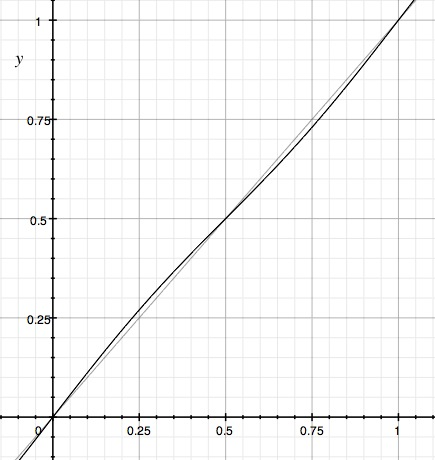
\includegraphics[scale=0.4]{sinewave}
\end{center}

\noindent Note that the two lines intersect at three points: \((0, 0), (\nicefrac{1}{2}, \nicefrac{1}{2})\) and \((1, 1)\). So if my credence in \(p\) is either 0, \(\nicefrac{1}{2}\) or 1, then my judgment is ratifiable. Otherwise, it is not. So the ratifiability constraint says that for any \(p\) about a baseball game, my credence in \(p\) should be either 0, \(\nicefrac{1}{2}\) or 1. But that's crazy. It's easy to imagine that I know (a) that in a particular game, the home team is much stronger than the away team, (b) that the stronger team usually, but far from always, wins baseball games, and (c) I'm systematically a little over-confident about my judgments about baseball games, in the way just described. In such a case, my credence that the home team will win should be high, but less than 1. That's just what the ratificationist denies is possible.

This kind of case proves that it isn't always rational to have ratifiable credences. It would take us too far afield to discuss this in detail, but it is interesting to think about the comparison between the kind of case I just discussed, and the objections to backwards induction reasoning in decision problems that have been made by Pettit and Sugden, and by Stalnaker. The backwards induction reasoning they criticise is, I think, a development of the idea that decisions should be ratifiable. And the clearest examples of when that reasoning fails concern cases where there is a unique ratifiable decision, and it is guaranteed to be one of the worst possible outcomes. The example I described in the last few paragraphs has, quite intentionally, a similar structure.

\subsection{A Privileged Stopping Point}

The other way to avoid the regress is to say that there is something special about the first level. So although \(J\) screens \(E\), it isn't the case that \(J^\prime\) screens \(J\). That way, the regress doesn't start. This kind of move is structurally like the move Adam Elga makes in \href{http://philsci-archive.pitt.edu/archive/00003702/}{How to Disagree about How to Disagree}, where he argues that we should adjust our views about first-order matters in (partial) deference to our peers, but we shouldn't adjust our views about the right response to disagreement in this way.

It's hard to see what could motivate such a position, either about disagreement or about screening. It's true that we need some kind of stopping point to avoid these regresses. But the most natural stopping point is the very first level. Consider a toy example. It's common knowledge that there are two apples and two oranges in the basket, and no other fruit. (And that no apple is an orange.) Two people disagree about how many pieces of fruit there are in the basket. \(A\) thinks there are four, \(B\) thinks there are five, and both of them are equally confident. Two other people, \(C\) and \(D\), disagree about what \(A\) and \(B\) should do in the face of this disagreement. All four people regard each other as peers. Let's say \(C\)'s position is the correct one (whatever that is) and \(D\)'s position is incorrect. Elga's position is that \(A\) should partially defer to \(B\), but \(C\) should not defer to \(D\). This is, intuitively, just back to front. \(A\) has evidence that immediately and obviously entails the correctness of her position. \(C\) is making a complicated judgment about a philosophical question where there are plausible and intricate arguments on each side. The position \(C\) is in is much more like the kind of case where experience suggests a measure of modesty and deference can lead us away from foolish errors. If anyone should be sticking to their guns here, it is \(A\), not \(C\).

The same thing happens when it comes to screening. Let's say that \(A\) has some evidence that (a) she has made some mistakes on simple sums in the past, but (b) tends to massively over-estimate the likelihood that she's made a mistake on any given puzzle. What should she do? One option, in my view the correct one, is that she should believe that there are four pieces of fruit in the basket, because that's what the evidence obviously entails. Another option is that she should be not very confident there are four pieces of fruit in the basket, because she makes mistakes on these kinds of sums. Yet another option is that she should be pretty confident (if not completely certain) that there are four pieces of fruit in the basket, because if she were not very confident about this, this would just be a manifestation of her over-estimation of her tendency to err. The `solution' to the regress we're considering here says that the second of these three reactions is the uniquely rational reaction. The idea behind the solution is that we should respond to the evidence provided by first-order judgments, and correct that judgment for our known biases, but that we shouldn't in turn correct for the flaws in our self-correcting routine. I don't see what could motivate such a position. Either we just rationally respond to the evidence, and in this case just believe there are four pieces of fruit in the basket, or we keep correcting for errors we make in any judgment. It's true that the latter plan leads either to regress or to the kind of ratificationism we dismissed in the previous subsection. But that's not because the disjunction is false, it's because the first disjunct is true.

\section{Conclusion}
We started with five related theses that are all closely tied to JSE. These are:

\begin{itemize}
\item The Equal Weight View of disagreement;
\item Roger White's anti-permissiveness epistemology;
\item David Christensen's conception of self-information as `higher-order evidence';
\item Andy Egan and Elga's view of the effects of knowledge of self-unreliability; and
\item Richard Feldman's view that we should `Respect the evidence'.
\end{itemize}

\noindent Not all of these views depend on JSE, but they're all supported in ways that I think rely on JSE. And some of them, mostly clearly the first, seem to be false if JSE is false. So JSE is deeply implicated in an important branch of contemporary epistemology. Yet JSE is false, as the last three sections have shown. This suggests that many of the positions on this branch have to be rethought.

The failure of JSE suggests a kind of externalism, though not of the traditional kind. It does not suggest, or at least does not require, that evidence be individuated in ways in principle inaccessible to the agent. It does not suggest, or at least does not require, that the force of evidence be determined by contingent matters, such as the correlation between evidence of this type and various hypotheses. But it does suggest that there are facts about which hypotheses are supported by which pieces of evidence, and that rational agents do well when they respond to these epistemic facts. Moreover, it suggests these facts retain their normative significance even if the agent has reason to believe that she's made a mistake in following them. That is, if an agent's judgment conforms to the correct norms of judgment, then even if she has evidence that she is not good at judging, she should stick to her judgment. In such a case she could not defend her judgment without appeal to the evidence that judgment is based on. But that's not a bad position to be in; judgments should be defensible by appeal to the evidence they're based on.
